\documentclass[a4paper,12pt]{exam}
\usepackage[utf8]{inputenc}
\usepackage[brazil]{babel}
\usepackage{graphicx,float,enumitem,multicol,array}
\usepackage{wrapfig,subfig}


\usepackage{mdframed}
\usepackage[most]{tcolorbox}

\usepackage{hyperref}
\usepackage{mathtools,icomma}
\usepackage{tcolorbox}
\usepackage{xcolor,colortbl}
\usepackage{amsfonts,amssymb}
\usepackage{pdfpages}
\usepackage[makeroom]{cancel} % símbolo de cancelar

% Configuração da lista
\newcommand{\instituicao}{ITA}
\newcommand{\campus}{São José dos Campos}
\newcommand{\curso}{Engenharia Eletrônica}
\newcommand{\materia}{Controle Clássico I}
\newcommand{\siglaMateria}{EES-10}
\newcommand{\professor}{José Roberto Colombo Junior}
\newcommand{\email}{colombojrcj@ita.br}

% Configuração dos cabeçalhos e rodapés
\lhead{\siglaMateria}
\chead[\bfseries\large Roteiro]{}
\rhead[\instituicao]{}
\footer{\curso}{}{Página \thepage\ de \numpages}

% Configurações diversas
\usepackage[bottom=4cm,top=2cm,left=1.5cm,right=1.5cm]{geometry}
\newcolumntype{L}[1]{>{\raggedright\let\newline\\\arraybackslash\hspace{0pt}}m{#1}}
\newcolumntype{C}[1]{>{\centering\let\newline\\\arraybackslash\hspace{0pt}}m{#1}}
\newcolumntype{R}[1]{>{\raggedleft\let\newline\\\arraybackslash\hspace{0pt}}m{#1}}
\pointpoints{ ponto}{ pontos}
\renewcommand{\solutiontitle}{\noindent\textbf{The solution:}\enspace}

% Custom colors
\usepackage{color}
\definecolor{deepblue}{rgb}{0,0,0.5}
\definecolor{deepred}{rgb}{0.6,0,0}
\definecolor{deepgreen}{rgb}{0,0.5,0}
\newcommand{\vermelho}[1]{{\textcolor{red}{#1}}}
\definecolor{verde}{rgb}{0,0.5,0}
\definecolor{verde_importante}{rgb}{0.2,0.75,0.65}

% Ambiente cuidado
% \newmdenv[linewidth=2pt,linecolor=orange,frametitle={\includegraphics[width=0.8cm]{figs/warning.pdf} Cuidado!}]{cuidado}

% Ambiente importante
\newmdenv[linewidth=2pt,linecolor=orange,frametitle={\includegraphics[width=0.8cm]{figs/importante.pdf} Importante!}]{importante}

\newtcbtheorem{pergunta}{\color{white} \bfseries Pergunta}{enhanced,drop shadow={black!50!white},
    coltitle=black,
    colback={blue!10},
    top=0.3in,
    attach boxed title to top right=
    {xshift=0em,yshift=-\tcboxedtitleheight/2},
    boxed title style={size=small,colback=blue}
}{Pergunta}

\newtcbtheorem{cuidado}{\color{white} \bfseries Cuidado}{enhanced,drop shadow={black!50!white},
    coltitle=black,
    colback={orange!10},
    top=0.3in,
    attach boxed title to top right=
    {xshift=0em,yshift=-\tcboxedtitleheight/2},
    boxed title style={size=small,colback=orange}
}{Cuidado}

%%%
% Default fixed font does not support bold face
\DeclareFixedFont{\ttb}{T1}{txtt}{bx}{n}{12} % for bold
\DeclareFixedFont{\ttm}{T1}{txtt}{m}{n}{12}  % for normal

% Configurando layout para mostrar codigos Python
\usepackage{listings}
\lstset{
  language=Python,
  basicstyle=\ttfamily\small,
  keywordstyle=\color{blue},
  stringstyle=\color{verde},
  commentstyle=\color{red},
  extendedchars=true,
  showspaces=false,
  showstringspaces=false,
  numbers=left,
  numberstyle=\tiny,
  breaklines=true,
  backgroundcolor=\color{green!10},
  breakautoindent=true,
  captionpos=b,
  xleftmargin=0pt,
}

% Python environment
\lstnewenvironment{python}[1][]
{
\pythonstyle
\lstset{#1}
}
{}

% Python for external files
\newcommand\pythonexternal[2][]{{
\pythonstyle
\lstinputlisting[#1]{#2}}}

% Python for inline
\newcommand\pythoninline[1]{{\pythonstyle\lstinline!#1!}}
%%%


\begin{document}

\begin{center}
  {\large \textbf{}} \\
  \vspace{5mm}
  
  \begin{tabular}{L{55mm}L{20mm}L{90mm}}\hline
    \includegraphics[width=50mm]{figs/logo.png}
    &     
    Disciplina: 
    
    Prof.

    Contato
    &
    \materia
    
    \professor

    \email
    \\ \hline
    
    Nome: \vspace*{8mm} & & \\ \hline
    Nome: \vspace*{8mm} & & \\ \hline
    Nome: \vspace*{8mm} & & \\ \hline
    Data: \vspace*{8mm} & & \\ \hline
%     Kit:  \vspace*{8mm} & & \\ \hline
  \end{tabular}
  
  \bigskip
\end{center}

\begin{cuidado}{}{}
    Os dispositivos usados podem causar acidentes!
\end{cuidado}

\section{Objetivos}

Nesse experimento serão estudados os seguintes tópicos:

\begin{itemize}
%     \item Obtenção do modelo do conjunto \textbf{motor + esc} (em torno de um ponto de operação)
    \item Obtenção do modelo do \textbf{aeropêndulo }(em torno de um ponto de operação)
%     \item Validação dos modelos do conjunto \textbf{motor + esc} e do \textbf{aeropêndulo} (em torno de um ponto de operação)
\end{itemize}

\section*{Formulário}

\begin{itemize}
    \item Máximo sobre-sinal $M_p = 100 e^{\frac{-\pi \xi}{\sqrt{1 - \xi^2}}}$ e $\xi = \frac{-\ln(M_p)}{\sqrt{\pi^2 + ln^2(M_p)}}$
    
    \item Tempo de estabelecimento $t_s = \dfrac{4}{\xi \omega_n}$ (critério de 2\%) e tempo de pico é $t_p = \frac{\pi}{\omega_n \sqrt{1 - \xi^2}}$
    
    \item FT característica de sistema de segunda ordem: $G(s) = \dfrac{K \omega_n^2}{s^2 + 2 \xi \omega_n s + \omega_n^2}$
    
    \item Erro em regime permanente para sistema de primeira ordem com controlador proporcional e realimentação unitária: $e_{ss} = \dfrac{1}{1 + K K_p}$
\end{itemize}


\newpage

\section{Procedimento de partida}

\begin{wrapfigure}[10]{l}{0.6\textwidth}
    \centering
    \vspace*{5mm}
    \includegraphics[width=8cm]{figs/sinal_partida.png}
    \caption{Solução do sinal de partida.}
    \label{fig:solucao-sinal-partida}
    
    \vspace*{5mm}
    \includegraphics[width=9cm]{figs/simulink_signal_builder.png}
    \caption{Sugestão de como deixar o diagrama de blocos (alto nível).}
    \label{fig:sugestao-diagrama-blocos-inicial}
    
\end{wrapfigure}

A partida do ESC+motor consiste em aplicar os passos descritos a seguir. Uma possível solução é apresentada na Figura \ref{fig:solucao-sinal-partida}.

\begin{enumerate}
    \item Habilitar a chave eletrônica: escreva 1 no pino PC15
    \item Esperar 0,5 segundos para a eletrônica do ESC inicializar
    \item Aplicar PWM com $t_{on}$ de 2000$~\mu$s
    \item Esperar 2 segundos
    \item Aplicar PWM com $t_{on}$ de 0$~\mu$s
    \item Esperar 4 segundos
    \item Aplicar PWM com $t_{on}$ de 1040$~\mu$s
    \item Esperar 3,5 segundos
    \item Aplicar $t_{on} = 0~\mu$s até o final do experimento
\end{enumerate} 

% \begin{wrapfigure}{l}{0.6\textwidth}
% \end{wrapfigure}

\hspace*{1mm}

Utilize o bloco \textit{Signal Builder} para construir o sinal de partida. Crie dois sinais nesse bloco. Um deles é o $partida(t)$, aplicado diretamente na planta durante a fase de inicialização. Essa fase tem duração de 10 segundos. Depois, o outro sinal $u(t)$ é o sinal de controle.

Vale lembrar que não aplicamos $u(t)$ no hardware. Ele aceita apenas \textit{duty cycle} $d(t)$. Para isso selecionaremos uma função que mapeia nosso sinal de controle $0 \leq u(t) \leq 100$ para $1040 \leq t_{on}(t) \leq 2000$ e então convertemos $t_{on}(t)$ para $d(t)$:

\begin{equation}
    t_{on}(t) = 1040 + \frac{960}{100} u(t)
\end{equation}

\begin{equation}
    d(t) = \frac{400}{10^6} t_{on}(t)
\end{equation}

Uma possível solução que combina os sinais de controle e partida é apresentada na Figura \ref{fig:solucao-sinal-controle}.

\begin{figure}[H]
    \centering
    \includegraphics[width=14cm]{figs/solucao_dac1.png}
    \caption{Solução do sinal de controle.}
    \label{fig:solucao-sinal-controle}
\end{figure}


\section{Leitura do sinal de posição angular}

Conforme conversamos no primeiro encontro de laboratório, o encoder é o sensor utilizado para medir a posição angular da haste do aeropêndulo. Quando configurado na resolução máxima, o encoder produz 8000 bordas a cada 360 graus. Logo, o ganho é $360 / 8000$ para converter para graus ou $2\pi / 8000$ para produzir radianos.

\begin{figure}[H]
    \centering
    \includegraphics[width=14cm]{figs/solucao_dac2.png}
    \caption{Solução para leitura do sinal do \textit{encoder}.}
    \label{fig:solucao-sinal-encoder}
\end{figure}

Depois do procedimento de partida, provavelmente o encoder não marca zero. Porém, utilizaremos essa posição angular como zero. Para isso, deve-se amostrar o sinal do encoder, guardá-lo e subtrair da sua respetiva leitura. Uma possível solução é mostrada na figura acima.

\newpage


\section{Modelo do aeropêndulo}

\begin{wrapfigure}[16]{l}{0.4\textwidth}
    \centering
    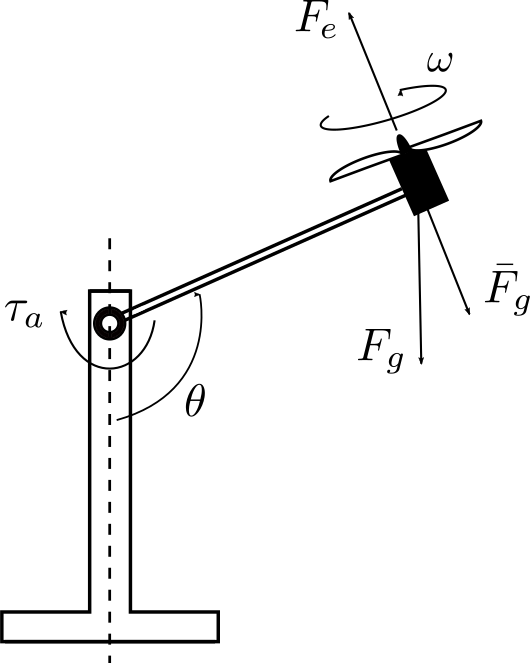
\includegraphics[width=5cm]{figs/aeropendulo/fig.pdf}
    \caption{Representação esquemática do aeropêndulo.}
    \label{fig:esquematico-aeropendulo}
\end{wrapfigure}


Após o processo de modelagem, verifica-se que a EDO que representa o comportamento deste sistema é não-linear:
%
\begin{equation}
  \label{eq:edo-original-nao-linear}
  \ddot{\theta}(t) = -\alpha \sin(\theta(t)) - \beta \dot{\theta}(t) + \gamma \omega^2(t)
\end{equation}

\noindent sendo $\alpha$, $\beta$ e $\gamma$ os parâmetros do modelo que precisam ser determinados e $\theta(t)$ e $\omega(t)$ a posição angular da haste e a velocidade do motor. Precisamos validar o modelo \eqref{eq:edo-original-nao-linear}. Iniciaremos levantando a curva estática do sistema.

Com base na equação \eqref{eq:edo-original-nao-linear}, se fizermos $\dot{\theta}(t) = \ddot{\theta}(t) = 0$, então

\begin{equation}
    \sin(\theta(t)) = \frac{\gamma}{\alpha} \omega^2(t)
\end{equation}

Note que essa relação só vale para valores estacionários.

\vspace*{5mm}
\subsection{Curva estática}

Qual o tipo de gráfico que você espera obter para a curva estática? Quadrático? Cúbico? Linear?

\makeemptybox{\stretch{1}}

O procedimento para levantar a curva estática é o seguinte: 

\begin{enumerate}
    \item Aplicar um sinal de controle constante ($u_{ss}$)
    \item Aguardar o transitório acabar
    \item Medir a saída ($y_{ss}$)
    \item Repetir os itens 1, 2 e 3 (com diferentes $u_{ss}$) para formar um gráfico
\end{enumerate}

\begin{cuidado}{}{}
    A curva estática só vale para pontos de equilíbrio \textbf{\underline{estáveis}}!
\end{cuidado}

\newpage

\begin{table}[H]
    \centering
    \begin{tabular}{C{2cm}|C{2cm}|C{2cm}|C{2cm}}
        \hline
        $u_{ss}$ & $y_{ss}$     & $y_{ss}$     & $y_{ss}$     \\ \hline
         5\%     & \vspace{1cm} & \vspace{1cm} & \vspace{1cm} \\ \hline
        10\%     & \vspace{1cm} & \vspace{1cm} & \vspace{1cm} \\ \hline
        15\%     & \vspace{1cm} & \vspace{1cm} & \vspace{1cm} \\ \hline
        20\%     & \vspace{1cm} & \vspace{1cm} & \vspace{1cm} \\ \hline
        25\%     & \vspace{1cm} & \vspace{1cm} & \vspace{1cm} \\ \hline
        30\%     & \vspace{1cm} & \vspace{1cm} & \vspace{1cm} \\ \hline
        35\%     & \vspace{1cm} & \vspace{1cm} & \vspace{1cm} \\ \hline
        40\%     & \vspace{1cm} & \vspace{1cm} & \vspace{1cm} \\ \hline
    \end{tabular}
\end{table}

Plote o gráfico referente aos valores obtidos. Em seguida responda:

\begin{enumerate}
    \item O resultado experimental bate com o esperado com o modelo teórico?
    \item O ESC é apenas um ganho? Em caso negativo, qual a função matemática que o ESC implementa?
    \item Apresente o polinômio de primeira ordem que mapeia $u_{ss}$ para $y_{ss}$
\end{enumerate}

\makeemptybox{\stretch{1}}

\newpage

Aplicando a linearização de Taylor à EDO \eqref{eq:edo-original-nao-linear}, chega-se na seguinte função de transferência:
%
\begin{equation}
  \label{eq:modelo-linear-aeropendulo}
  \frac{\Delta \theta(s)}{\Delta U(s)} = \frac{\gamma}{s^2 + \beta s + \alpha \cos(\bar{\theta})}
\end{equation}

\noindent que vale apenas em torno do ponto de operação $(\bar{u}, \bar{\theta})$.

Realize ensaios experimentais para determinar os parâmetros $\alpha$, $\beta$ e $\gamma$ da função de transferência (que deveriam bater com os do modelo não-linear) para os pontos de operação:

\begin{table}[H]
    \centering
    \begin{tabular}{C{2cm}|C{2cm}}
        \hline
        $\bar{y}$ & $\bar{u}$    \\ \hline
        20\%      & \vspace{1cm} \\ \hline
        40\%      & \vspace{1cm} \\ \hline
    \end{tabular}
\end{table}

\begin{cuidado}{}{}
    Implemente uma rampa \textbf{suave} para levar o sistema até o ponto de operação.
\end{cuidado}

Descreva o procedimento que a sua dupla/trio utilizou para obter os parâmetro e em seguida, apresente os parâmetros.

\makeemptybox{\stretch{1}}

\newpage


\end{document}


